\themaM
\graphicspath{{../../S19_Volumes_et_capacites/Images/}}

\chapter{Volumes et capacités}
\label{S19}


%%%%%%%%%%%%%%%%%%%%%%%%%%%%%%%%%%%%%%%%%%
%%%%%%%%%%%%%%%%%%%%%%%%%%%%%%%%%%%%%%%%%%
\begin{prerequis}
   \begin{itemize}
      \item Calculer le volume d'un prisme, d'un cylindre.
      \item Correspondance entre volume et contenance : \\
         $\ul{1} =\udmc{1}$ et $\ul{1000} =\umc{1}$.
      \item[\com] Mener des calculs impliquant des grandeurs mesurables, notamment des grandeurs composées, exprimer les résultats dans les unités adaptées.
      \item[\com] Vérifier le cohérence des résultats au niveau des unités.
      \item[\com] Effectuer des conversions d'unités de volumes.
   \end{itemize}
\end{prerequis}

\vfill

\begin{debat}[Débat : $\ul{1} =\udmc{1}$]
   Cette correspondance est à connaître. Pourtant, elle ne paraît pas si naturelle que cela : elle signifie que l'eau contenue dans une bouteille d'un litre remplirait exactement un cube de \udm{1} de côté.
   \begin{center}
      \begin{pspicture}(0,-0.25)(6,5.5)
         \psline(0.5,0.5)(0.5,3.75) %bouteille
         \psline(2,0.5)(2,3.75)
         \psarc(1.5,3.75){0.5}{0}{90}
         \psarc(1,3.75){0.5}{90}{180}
         \psline(1,4.25)(1,5)
         \psline(1.5,4.25)(1.5,5)
         \psellipticarc(1.25,0.5)(0.75,0.3){180}{0}
         \psellipticarc(1.25,3.5)(0.75,0.3){180}{0}
         \psellipticarc[linestyle=dashed](1.25,3.5)(0.75,0.3){0}{180}
         \psellipse(1.25,5)(0.25,0.1)
         \rput(1.25,2){\textcolor{B1}{\ul{1}}}
         \psframe(3,0.5)(5,2.5) %cube
         \psline(3,2.5)(3.75,3.25)(5.75,3.25)(5.75,1.25)(5,0.5)
         \psline(5,2.5)(5.75,3.25)
         \rput(4,0.2){\textcolor{B1}{$\udm{1} =\ucm{10}$}}
         \rput(4,1.5){\textcolor{B1}{$\udmc{1}$}}
      \end{pspicture}
   \end{center}
   \bigskip
   \begin{cadre}[B2][F4]
      \begin{center}
         Vidéo : \href{https://www.youtube.com/watch?v=DRKmlWtUN0k}{\bf Correspondance entre unités de volume et de contenance}, chaîne YouTube de {\it Jean-Charles Toussaint}.
      \end{center}
   \end{cadre}
\end{debat}

\vfill

\textcolor{PartieGeometrie}{\sffamily\bfseries Cahier de compétences} : chapitre 12, exercices 24 à 42.


%%%%%%%%%%%%%%%%%%%%%%%%%%%%%%%%%%%%
%%%%%%%%%%%%%%%%%%%%%%%%%%%%%%%%%%%%
\activites

\begin{activite}[Des pavés de toutes sortes]
   {\bf Objectifs :} calculer le volume d'un pavé ; différencier volume et capacité ; résoudre un problème dans le domaine des grandeurs et mesures.
   \begin{QCM}
      \partie[observations]
         Quelle action est matérialisée par le schéma suivant ? \\ [2mm]
         \pf \\ [2mm]
         \pf \\
         \begin{center}
            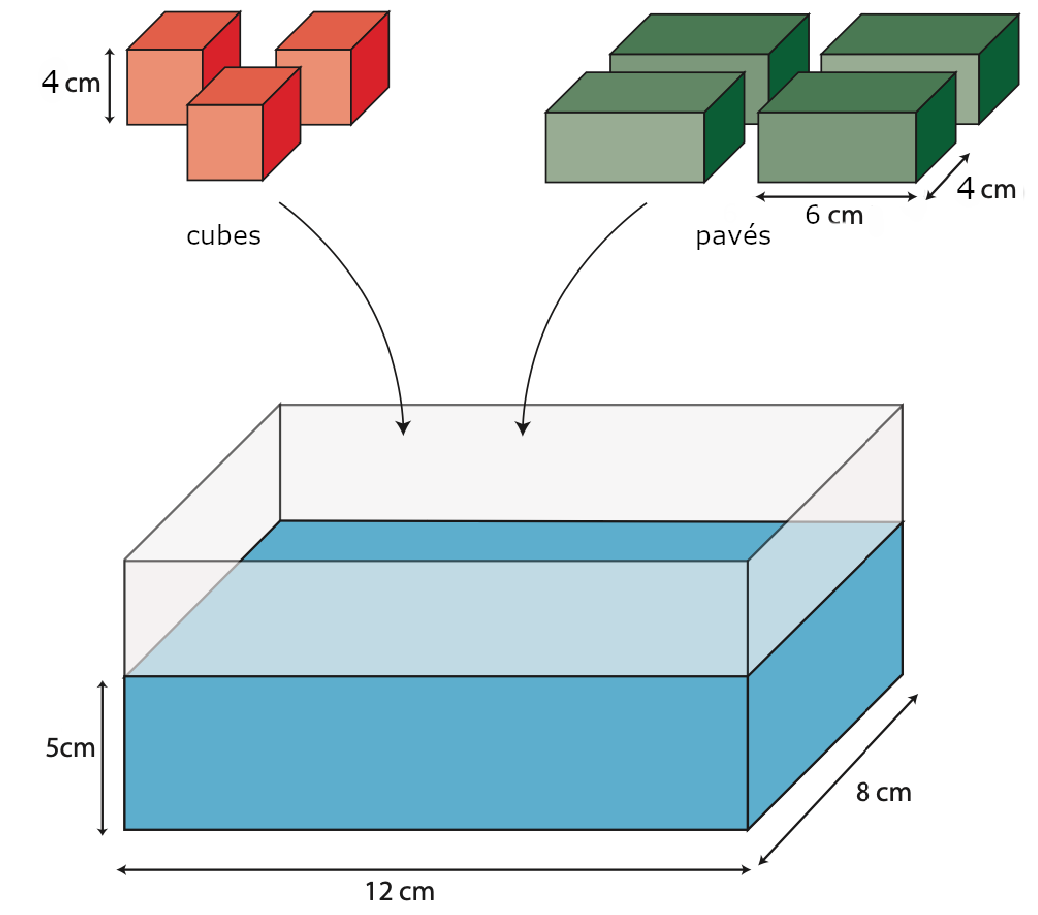
\includegraphics[width=8cm]{piscine}
         \end{center}
      \partie[questions]
         \begin{enumerate}
            \item Quel est le volume d'eau en \ucmc{} contenu dans la boite transparente ? \\ [2mm]
               \pf \\
            \item Quelle est la capacité d'eau en L contenue dans la boite transparente ? \\ [2mm]
               \pf \\
            \item Dans la bassine, on plonge trois cubes et quatre pavés. Quelle doit être la hauteur des pavés pour que l'eau monte de \ucm{4} ? \\ [2mm]
               \pf \\ [2mm]
               \pf \\ [2mm]
               \pf
         \end{enumerate}
      \end{QCM}
      \vfill \hfill {\it\footnotesize Source : d'après l'activité \href{http://www-irem.univ-paris13.fr/site_spip/IMG/pdf/des_paves_dans_la_mare_2_noir.pdf}{Des pavés dans la mare}, IREM Paris Nord.}
\end{activite}


%%%%%%%%%%%%%%%%%%%%%%%%%%%%%%%%%%%%%%%%%%
%%%%%%%%%%%%%%%%%%%%%%%%%%%%%%%%%%%%%%%%%%
\cours 

\section{Volume par dénombrement} %%%%%%%%%%%%%%%%%%%%%

\begin{definition}
   Le \textbf{volume} est une grandeur physique qui mesure l'espace occupé par celui-ci.
\end{definition}

\begin{exemple*1}
   {\psset{unit=0.5}
   Ces trois objets n'ont pas la même forme mais occupent la même quantité d'espace, ils ont donc le même volume. \\
   \begin{minipage}{8cm}
      \begin{pspicture}(0,-1)(13,3.8)
         \psset{linecolor=A1}
         \psframe(0,0)(3,2)
         \psline(1,0)(1,2)(1.5,2.5)
         \psline(2,0)(2,2)(2.5,2.5)
         \psline(0,1)(3,1)(3.5,1.5)
         \psline(3,0)(3.5,0.5)(3.5,2.5)(0.5,2.5)(0,2)
         \psline(3,2)(3.5,2.5)
         \psset{linecolor=B1}
         \pspolygon(5,0)(9,0)(9,2)(8,2)(8,1)(6,1)(6,2)(5,2)
         \psline(5,1)(6,1)(6,0)
         \psline(7,0)(7,1)(7.5,1.5)
         \psline(9,0)(9.5,0.5)(9.5,2.5)(8.5,2.5)(8,2)
         \psline(9,2)(9.5,2.5)
         \psline(9.5,1.5)(9,1)(8,1)(8,0)
         \psline(5,2)(5.5,2.5)(6.5,2.5)(6.5,1.5)(8,1.5)
         \psline(6,2)(6.5,2.5)
         \psline(6,1)(6.5,1.5)    
         \psset{linecolor=G1}  
         \pspolygon(11,0)(14,0)(14,1)(13,1)(13,2)(12,2)(12,3)(11,3)
         \psline(12,0)(12,1)(11,1)
         \psline(13,0)(13,1)(12,1)(12,2)(11,2)
         \psline(14,0)(14.5,0.5)(14.5,1.5)(13.5,1.5)(13.5,2.5)(12.5,2.5)(12.5,3.5)(11.5,3.5)(11,3)
         \psline(14,1)(14.5,1.5)
         \psline(13,2)(13.5,2.5)
         \psline(12,3)(12.5,3.5)
         \psline(13,1)(13.5,1.5)
         \psline(12,2)(12.5,2.5)
      \end{pspicture}
   \end{minipage}
   \begin{minipage}{5cm}
   Si l'unité de volume est un cube \, \psline(0,1)(0,0)(1,0)(1,1)(0,1)(0.5,1.5)(1.5,1.5)(1.5,0.5)(1,0) \psline(1,1)(1.5,1.5) \\
   le volume de ces trois solides est de 6 unités de volume.
   \end{minipage}}
\end{exemple*1}

\bigskip

Il existe deux unités en dimension 3 : les unités de volumes en \og cube \fg{} et les unités de capacité en \og litre \fg. 

\begin{definition}
   \begin{itemize}
      \item Lorsque l'unité de volume est un cube de \um{1} d'arête, cela représente \umc{1}.
      \item Le {\bf litre} (L) est une unité de capacité valant \udmc{1}. On a alors $\ul{1} =\udmc{1}$ et $\ul{1000} =\umc{1}$.
   \end{itemize}
   \ \\ [-12mm]
\end{definition}

\bigskip

Pour effectuer un changement d'unité de volume, on reprend les même préfixes que pour les changements de longueur, et on impose pour chacun d'eux trois colonnes au tableau.
\begin{center}
   {\hautab{1.3}
      \begin{ltableau}{0.9\linewidth}{21}
         \hline
         \multicolumn{3}{|c|}{\ukmc{}}
         & \multicolumn{3}{c|}{\uhmc{}}
         & \multicolumn{3}{c|}{\udamc{}}
         & \multicolumn{3}{c|}{\umc{}}
         & \multicolumn{3}{c|}{\udmc{}}
         & \multicolumn{3}{c|}{\ucmc{}}
         & \multicolumn{3}{c|}{\ummc{}} \\
         \hline
         & & & & & & & 2 & 1 & 0 & 9 & 2 & 8 & 0 & 1 & 5 & & & & & \\
         \hline
      \end{ltableau}}
\end{center}

\smallskip

Ainsi, pour convertir d'une unité à l'autre; on multiplie ou on divise par \numprint{1000}, \numprint{1000000}\dots

\begin{exemple*1}
    \udamc{21,092801\,5} = \umc{21092,8015} = \udmc{21092801,5}  = \ucmc{21092801500}.
\end{exemple*1}
   
\section{Volumes classiques} %%%

\begin{center}
\begin{tabular}{p{5cm}|p{5cm}|p{5cm}}
   {\bf Le pavé droit} : ${\cal V}=L\times \ell\times h$
   & {\bf Le prisme} : ${\cal V}={\cal A}\times h$
   & {\bf Le cylindre} : ${\cal V}=\pi\times r^2\times h$ \\
   \begin{center}
      \begin{pspicture}(-0.5,-0.5)(5,3)
         \pspolygon(0,0)(3,0)(4,1)(4,3)(1,3)(0,2)
         \psline(0,2)(3,2)(3,0)
         \psline(3,2)(4,3)
         \psline[linestyle=dashed](0,0)(1,1)(4,1)
         \psline[linestyle=dashed](1,1)(1,3)
         \psset{linecolor=B1}
         \psline{<->}(0,-0.3)(3,-0.3)
         \rput(1.5,-0.6){\textcolor{B1}{$L$}}
         \psline{<->}(-0.3,0)(-0.3,2)
         \rput(-0.6,1){\textcolor{B1}{$\ell$}}
         \psline{<->}(-0.2,2.2)(0.9,3.3)
         \rput(0.2,3){\textcolor{B1}{$h$}}
      \end{pspicture}
   \end{center}
   &
   \begin{center}
      \begin{pspicture}(-0.75,-0.5)(5,3)
         \psline(0,2)(1.5,3)(2.5,3)(3.5,2.5)(1,1.5)(0,2)(0,0.5)(1,0)(3.5,1)(3.5,2.5)
         \psline(1,0)(1,1.5)
         \psline[linestyle=dashed](0,0.5)(1.5,1.5)(2.5,1.5)(3.5,1)
         \psline[linestyle=dashed](1.5,1.5)(1.5,3)
         \psline[linestyle=dashed](2.5,1.5)(2.5,3)
         \psline[linecolor=B1]{<->}(-0.25,0.5)(-0.25,2)
         \rput(-0.55,1.25){\textcolor{B1}{$h$}}
         \rput(1.75,0.9){\textcolor{B1}{$\mathcal{A}$}}
      \end{pspicture}
   \end{center}
   &
   \begin{center}
      \begin{pspicture}(-0.5,0.5)(5,3.5)
         \psline(0.5,1)(3.5,1)
         \psline(0.5,3)(3.5,3) 
         \psellipse(3.5,2)(0.3,1) 
         \psellipticarc(0.5,2)(0.3,1){90}{-90}
         \psellipticarc[linestyle=dashed](0.5,2)(0.3,1){-90}{90}
         \psset{linecolor=B1}
         \psline{<->}(0.5,0.7)(3.5,0.7)
         \rput(2,0.35){\textcolor{B1}{$h$}}
         \psline{<->}(3.5,1)(3.5,2)
         \rput(3.65,1.6){\textcolor{B1}{$r$}}
      \end{pspicture}
   \end{center} \\
   Le {\bf cube} de côté $c$ est un cas particulier avec $L=\ell=h=c : {\cal V}=c^3$
   &
   $\cal A$ est l'aire d'une base, $h$ la hauteur du prisme.
   &
   $h$ est la hauteur du cylindre, $r$ est le rayon du disque de base.
   \\
\end{tabular}
\end{center}


%%%%%%%%%%%%%%%%%%%% %%%%%%%%%%%%%%%%%%%%
%%%%%%%%%%%%%%%%%%%% %%%%%%%%%%%%%%%%%%%%
\exercicesbase

\begin{colonne*exercice}

\serie{Calcul de volumes}

\begin{exercice} %1
   Donner le volume de chaque solide en unités de volume (les volumes sont supposés pleins).
   \begin{center}
      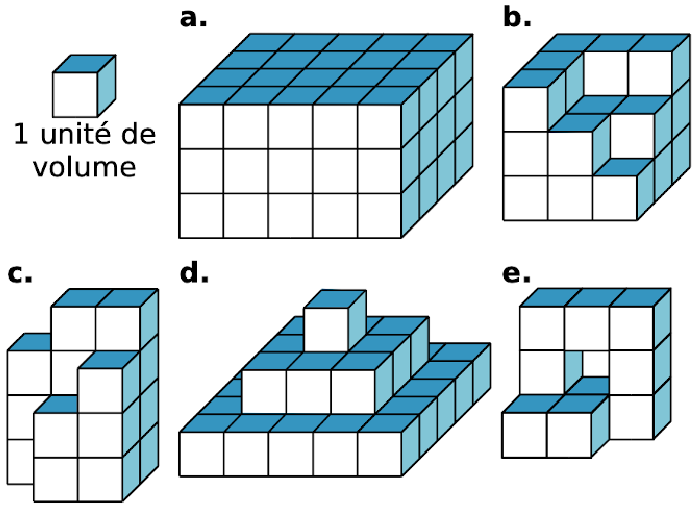
\includegraphics[width=7.5cm]{cubes}
   \end{center}
\end{exercice}

\begin{corrige}
  a. {\blue 60 u} \quad ; b. {\blue 22 u} \quad ; c. {\blue 16 u} \quad ; d. {\blue 35 u} \quad ; e. {\blue 10 u}
\end{corrige}



\begin{exercice} %2
   Dans chacune des figures suivantes, colorier une base en jaune, repasser une hauteur en rouge puis calculer le volume.
   \begin{center}
      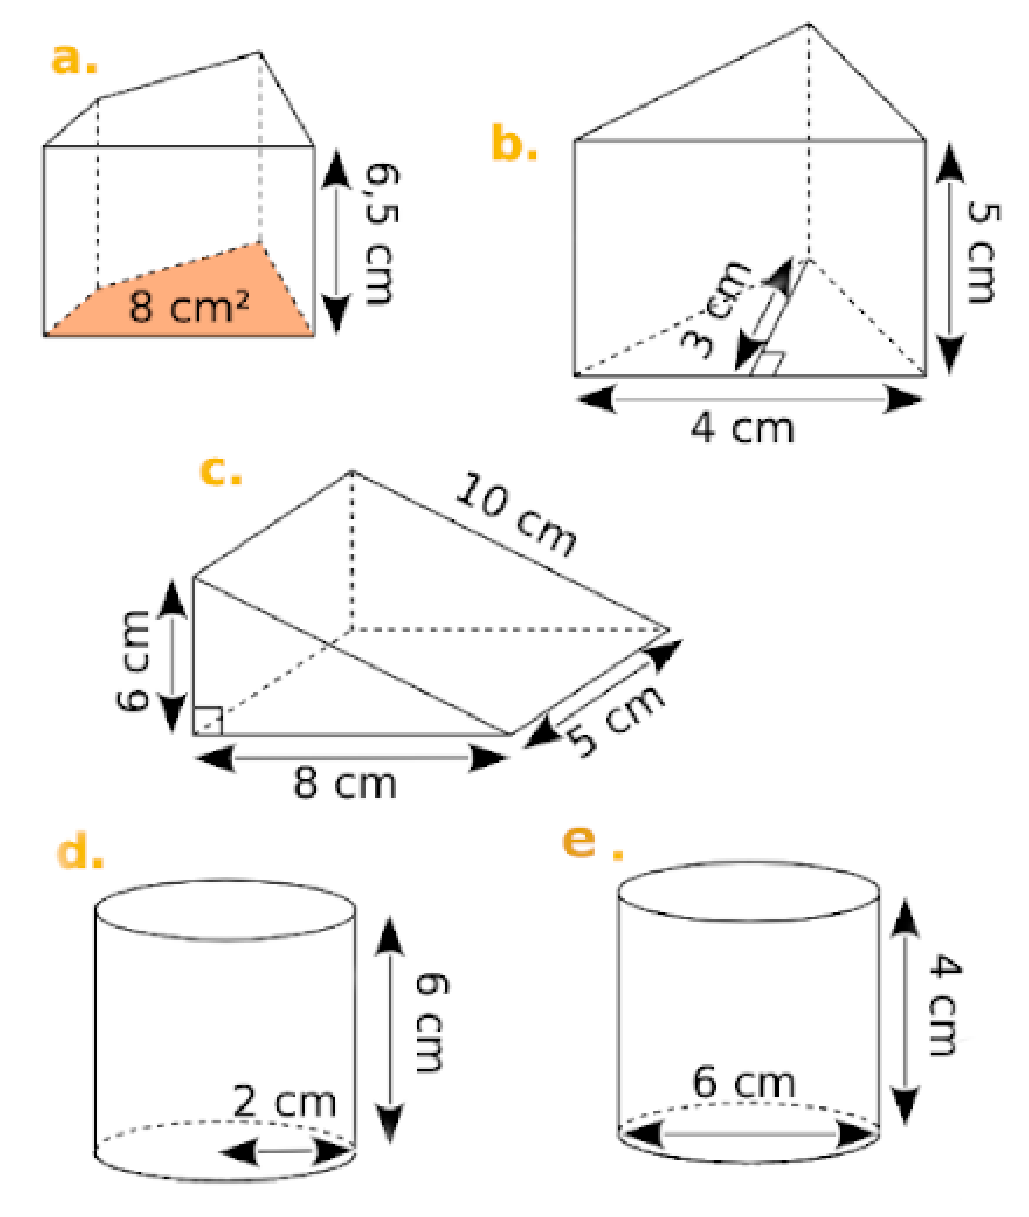
\includegraphics[width=8cm]{volumes_ex2}
   \end{center}
\end{exercice}

\begin{corrige}
   \begin{itemize}
      \item $V_a =\ucmq{8}\times\ucm{6,5} ={\blue \ucmc{52}}$ \smallskip
      \item $V_b =\dfrac{\ucm{4}\times\ucm{3}}{2}\times\ucm{5} ={\blue \ucmc{30}}$ \smallskip
      \item $V_c =\dfrac{\ucm{8}\times\ucm{6}}{2}\times\ucm{5} ={\blue \ucmc{120}}$ \smallskip
      \item $V_d =\pi\times(\ucm{2})^2\times\ucm{6} \approx{\blue \ucmc{75,4}}$ \smallskip
      \item $V_e =\pi\times(\ucm{3})^2\times\ucm{4} \approx{\blue \ucmc{113,1}}$
   \end{itemize}
\end{corrige}


\begin{exercice} %3
   Les figures colonne suivante représentent deux pièces d'un jeu. Comparer leur volume.
   \begin{center}
      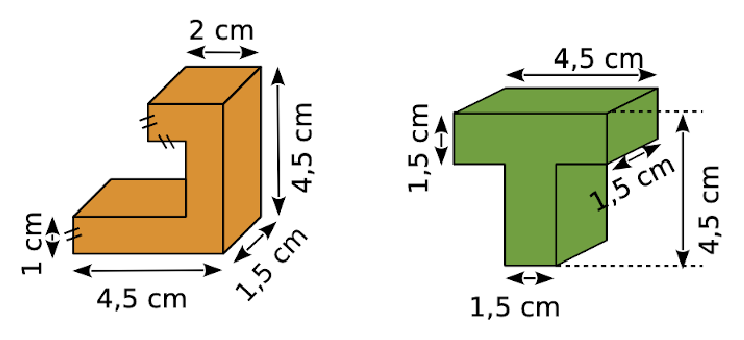
\includegraphics[width=8cm]{pieces}
   \end{center}
\end{exercice}

\begin{corrige}
   \begin{itemize}
      \item La première figure est composée de trois pavés droits : le \og pied \fg{} de mesures \ucm{1}; \ucm{4,5} et \ucm{1,5} ; le \og haut \fg{} de mesures \ucm{2}; \ucm{1} et \ucm{1,5} et enfin la partie qui relie les deux de mesures \ucm{1}; \ucm{2,5} et \ucm{1,5}. \\
      On calcule le volume en \ucmc{} : \\
      $1\times4,5\times1,5+2\times1\times1,5+1\times2,5\times1,5 ={\blue 13,5}$
      \item La deuxième figure est composée de deux pavés droits : le pied de mesures \ucm{1,5}; \ucm{1,5} et \ucm{3} et la tête de mesures \ucm{1,5}; \ucm{4,5} et \ucm{1,5}. \\
      Or, $1,5\times1,5\times3+1,5\times4,5\times1,5 ={\blue 16,875}$
      \item Donc, {\blue la deuxième pièce est la plus volumineuse}.
   \end{itemize}
\end{corrige}



\serie{Volumes et capacités : problèmes}

\bigskip


\begin{exercice} %4
   Pour un chantier, un maçon doit construire quatre colonnes en béton de forme cylindrique, de \ucm{50} de rayon et de \um{4} de hauteur.
   \begin{enumerate}
      \item Quel est le volume total des colonnes ?
      \item Pour \umc{1} de béton, il faut \ukg{400} de ciment, \ul{460} de sable, \ul{780} de gravillons et \ul{200} d'eau. \\
         Donner la quantité de ciment, de sable, de gravillons et d'eau nécessaire pour les quatre colonnes.
   \end{enumerate}
\end{exercice}

\begin{corrige}
   \ \\ [-5mm]
   \begin{enumerate}
      \item $V =4\times(\pi\times(\um{0,5})^2\times\um{4}) \approx \umc{12,57}$. \\
         {\blue Le volume des colonnes est d'environ \umc{12,57}}.
      \item Les valeurs sont pour \umc{1} donc, il suffit de multiplier toutes les quantités par 12,57 : \\
         Il faut $12,57\times\ukg{400} =$ {\blue \ukg{5028} de ciment} ; \\
         $12,57\times\ul{460} \approx$ {\blue \ul{5 782} de sable} ; \\
         $12,57\times\ul{780} \approx$ {\blue \ul{9 805} de gravillons} et \\
         $12,57\times\ul{200} =$ {\blue \ul{2 514} d'eau}.
   \end{enumerate}
\end{corrige}

\bigskip


\begin{exercice} %5
   Ilia dispose de deux seaux d'exactement 3 litres et 5 litres. Chaque seau a une forme cylindrique et l'aire de leur base est de \ucmq{200}.
   \begin{enumerate}
      \item Calcule la hauteur de chacun de ces seaux.
      \item Comment va procéder Ilia pour obtenir \ul{4} en utilisant uniquement ses seaux de \ul{3} et \ul{5} ?
   \end{enumerate}
\end{exercice}

\begin{corrige}
  \ \\ [-5mm]
  \begin{enumerate}
      \item Le volume d'un cylindre est égal à l'aire de sa base multipliée par la hauteur donc, pour trouver la hauteur, il suffit de diviser le volume par l'aire. \\
         Seau de \ul{3} : $h =\dfrac{\ul{3}}{\ucmq{200}} =\dfrac{\udmc{3}}{\udmq{2}} =\udm{1,5}$. \\ [1mm]
         Seau de \ul{5} : $h =\dfrac{\ul{5}}{\ucmq{200}} =\dfrac{\udmc{5}}{\udmq{2}} =\udm{2,5}$. \\ [1mm] 
      Les seaux ont une hauteur de {\blue \ucm{15} et \ucm{25}}.
   \end{enumerate}

\Coupe

   \begin{enumerate}
   \setcounter{enumi}{1}
      \item Remplir le seau de 5L, le verser dans celui de 3L \\
         -- vider le petit seau, et le remplir avec le grand qui contient \ul{2} \\
         -- remplir de nouveau le seau de \ul{5}, en verser une partie dans le petit qui contient \ul{2} \\
         -- il reste alors \ul{4} dans le gros seau.
   \end{enumerate}
\end{corrige}

\bigskip


\begin{exercice} %7
   Voici la représentation en perspective cavalière d'une maison de poupée dont les longueurs sont exprimées en centimètres.
   \begin{center}
      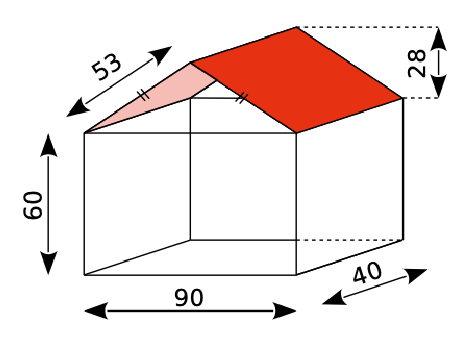
\includegraphics[width=6cm]{maison}
   \end{center}
   \ \\ [-12mm]
   \begin{enumerate}
      \item Calculer la surface de bois nécessaire pour réaliser le modèle de la maison.
      \item Sachant que le contre-plaqué choisi coûte \ueuro{28,90} le \umq{}, calculer le montant de sa dépense.
      \item Calculer, au \udmc{} près, le volume de la maison.
   \end{enumerate}
\end{exercice}

\begin{corrige}
   \ \\ [-5mm]
   \begin{enumerate}
      \item On a les pièces suivantes, les aires sont en \ucmq{} :
         \begin{itemize}
            \item fond : $90\times40 =3\,600$ ;
            \item face et arrière : $2\times(90\times60) =10\,800$ ;
            \item côtés : $2\times(40\times60) =4\,800$ ; 
            \item toit : $2\times(40\times53) =4\,240$ ; \smallskip
            \item pignons : $2\times\dfrac{90\times28}{2} =2\,520$. \smallskip
         \end{itemize}
         On additionne les mesures de toutes les pièces : \\
         $3\,600+10\,800+4\,800+4\,240+2\,520 =25\,960$. \\
         {\blue Il faut \ucmq{25960} de bois pour la maison}.
      \item $\ucmq{25960} =\umq{2,596}$ et $2,596\times28,90 \approx75,02$. \\
      {\blue Le montant sera d'environ \ueuro{75}}.
      \item La maison a la forme d'un prisme dont la base est une façade de mesure : \\
      \ucmq{5400} + \ucmq{1260} = \ucmq{6660} et dont la hauteur vaut \ucm{40}. Son volume est donc de $\ucmq{6660}\times\ucm{40} =\ucmc{266400} =\udmc{266,4}$. \\
      {\blue Le volume de la maison est d'environ \udmc{266}}.
   \end{enumerate}
   
\bigskip
\corec{Format A5 et cylindres}
\smallskip

\begin{enumerate}
   \setcounter{enumi}{4}
      \item Format A4 : {\blue $\ell =\ucm{21}; L=\ucm{29,7}$}. \\
         Format A5 : {\blue $\ell =\ucm{29,7}\div2 = \ucm{14,85}; L=\ucm{21}$}.
      \item
      \begin{enumerate}
         \item La hauteur vaut {\blue $h_1 =\ucm{14,85}$}.
         \item Le périmètre du disque vaut {\blue $P_1 =\ucm{21}$}. \\
         Or, le périmètre d'un disque se calcule grâce à la formule $2\pi\times R$ où $R$ est le rayon du disque. \\
            Donc,  ${\blue R_1} =\ucm{21}\div(2\pi) {\blue \approx\ucm{3,34}}$.
         \item $\mathcal{V}_1 =\pi\times R_1^2\times h_1 \approx\pi\times(\ucm{3,34})^2\times\ucm{14,85}$ \\
            {\blue $\mathcal{V}_1 \approx\ucmc{520,44}$}.
      \end{enumerate}
      \setcounter{enumi}{6}
      \item
      \begin{enumerate}
         \item La hauteur vaut {\blue $h_2 =\ucm{21}$}.
         \item Le périmètre du disque vaut {\blue $P_2 =\ucm{14,85}$}. \\
            Donc,  ${\blue R_2} =\ucm{14,85}\div(2\pi) {\blue \approx\ucm{2,36}}$.
         \item $\mathcal{V}_2 =\pi\times R_2^2\times h_2 \approx\pi\times(\ucm{2,36})^2\times\ucm{21}$ \\
            {\blue $\mathcal{V}_2 \approx\ucmc{367,45}$}.
      \end{enumerate}
      \setcounter{enumi}{7}
      \item {\blue Le premier cylindre a le volume le plus grand}, malgré la feuille identique.
   \end{enumerate}
\end{corrige}

\smallskip   
\hfill{\it\footnotesize Source : D’après Les cahiers Sésamath 5e. Magnard-Sesamath 2017}

\end{colonne*exercice}


%%%%%%%%%%%%%%%%%%%%%%%%%%%%%%%%%%%
%%%%%%%%%%%%%%%%%%%%%%%%%%%%%%%%%%%
\Recreation

\enigme[Format A5 et cylindres]
   \partie[construction de cylindres]
   \ \\ [-10mm]
      \begin{enumerate}
         \item Découper une feuille au format A4 suivant sa médiane la plus courte afin d'obtenir deux feuilles au format A5.
            \begin{center}
               \begin{pspicture}(0,0)(3,2.3)
                  \psframe(0,0)(3,2.1)
                  \psline[linestyle=dashed](1.5,0)(1.5,2)
                  \rput(0.75,1){A5}
                  \rput(2.25,1){A5}
               \end{pspicture}
            \end{center}
         \begin{multicols}{2}
         \item Rouler la première feuille dans le sens de la \\
            longueur pour former un premier cylindre. \\
            {\psset{unit=0.7}
               \begin{pspicture}(0.5,-0.5)(11,3.75)
                  \psframe(0,0)(3,2.1)
                  \rput(1.5,1){A5}
                  \rput(4,1){$\Rightarrow$}
                  \psline(5.6,-0.37)(5.6,1.65)
                  \psline(5,0)(5,2)
                  \psline(7,0)(7,2)
                  \psellipticarc(6,2)(1,0.4){0}{-137}
                  \psellipticarc(6,0)(1,0.4){0}{137}
                  \psellipticarc(6,0)(1,0.4){180}{-137}
                  \rput(8,1){$\Rightarrow$}
                  \psline(10.5,0)(10.5,2)
                  \psline(9,0)(9,2)
                  \psellipse(9.75,2)(0.75,0.3)
                  \psellipticarc(9.75,0)(0.75,0.3){180}{0}
               \end{pspicture}}
         \item Rouler la deuxième feuille dans le sens de la \\
            largeur pour former un deuxième cylindre. \\
            {\psset{unit=0.71}
               \begin{pspicture}(0,-0.5)(8.5,3.75)
                  \psframe(0,0)(2.1,3)
                  \rput(1,1.5){A5}
                  \rput(3,1.5){$\Rightarrow$}
                  \psline(4.4,-0.3)(4.4,2.7)
                  \psline(4,0)(4,3)
                  \psline(5.5,0)(5.5,3)
                  \psellipticarc(4.75,3)(0.75,0.35){0}{-137}
                  \psellipticarc(4.75,0)(0.75,0.35){0}{137}
                  \psellipticarc(4.75,0)(0.75,0.35){180}{-137}
                  \rput(6.5,1.5){$\Rightarrow$}
                  \psline(8.5,0)(8.5,3)
                  \psline(7.5,0)(7.5,3)
                  \psellipse(8,3)(0.5,0.25)
                  \psellipticarc(8,0)(0.5,0.25){180}{0}
               \end{pspicture}}
         \end{multicols}
         \item À votre avis, ces cylindres ont-il le même volume ? Si non, quel est celui qui semble avoir le volume le plus grand ? \pf \\
      \end{enumerate}
      
   \partie[calcul du volume]
   \ \\ [-10mm]
   \begin{enumerate}
     \setcounter{enumi}{4}
        \item Rappeler les dimensions d'une feuille au format A4. En déduire les dimensions d'une feuille au format A5. \\ [2mm]
           \pf \medskip
        \item Premier cylindre.
        \begin{enumerate}
           \item Donner la mesure de la hauteur du cylindre. \pf \\
           \item Que vaut le périmètre du disque de base du cylindre ? En déduire son rayon. \\ [2mm]
           \pf \medskip
           \item Calculer alors  le volume du premier cylindre. \\ [2mm]
           \pf \\
        \end{enumerate}
        \item Deuxième cylindre.
        \begin{enumerate}
           \item Donner la mesure de la hauteur du cylindre. \pf \\
           \item Que vaut le périmètre du disque de base du cylindre ? En déduire son rayon. \\ [2mm]
           \pf \medskip
           \item Calculer alors  le volume du deuxième cylindre. \\ [2mm]
           \pf \bigskip
        \end{enumerate}
        \item Conclusion : \pf
     \end{enumerate}

